\documentclass[10pt,twocolumn,letterpaper]{article}

\usepackage{cvpr}
\usepackage{times}
\usepackage{epsfig}
\usepackage{graphicx}
\usepackage{amsmath}
\usepackage{amssymb}

% Include other packages here, before hyperref.

% If you comment hyperref and then uncomment it, you should delete
% egpaper.aux before re-running latex.  (Or just hit 'q' on the first latex
% run, let it finish, and you should be clear).
\usepackage[breaklinks=true,bookmarks=false]{hyperref}

\cvprfinalcopy % *** Uncomment this line for the final submission

\def\cvprPaperID{****} % *** Enter the CVPR Paper ID here
\def\httilde{\mbox{\tt\raisebox{-.5ex}{\symbol{126}}}}

% Pages are numbered in submission mode, and unnumbered in camera-ready
%\ifcvprfinal\pagestyle{empty}\fi
% \setcounter{page}{4321}
\begin{document}

%%%%%%%%% TITLE
\title{Pushbroom satellite image super-resolution using generative adversarial networks}

\author{Chao Xu\\
The Chinese University of Hong Kong\\
Shatin, New Territories, Hong Kong SAR\\
{\tt\small 1155160618@lin.cuhk.edu.hk}
% For a paper whose authors are all at the same institution,
% omit the following lines up until the closing ``}''.
% Additional authors and addresses can be added with ``\and'',
% just like the second author.
% To save space, use either the email address or home page, not both
}
\maketitle
%\thispagestyle{empty}

%%%%%%%%% ABSTRACT
\begin{abstract}
In order to improve the resolution or visual effect of imageries from pushbroom sensors, this report proposes to use super-resolution generative adversarial networks (SRGAN)~\cite{ledig2017photo}. Some improvements are achieved: firstly, the VGG-19~\cite{simonyan2014very} network is modified to extract the features of input images, and thus reduce the training time; secondly, the loss function is updated as new evaluation metric for the generated images; finally, three models with different hyperparameters are trained and compared to find the optimal results. In this report,  the pushbroom image super-resolution is achieved with a scale factor of 4, and the result shows a better visual perception compared with that recovered by bicubic interpolation. We call the network model in this report as pbiSRGAN, which is Push-Broom Images SRGAN.         
\end{abstract}

%%%%%%%%% BODY TEXT
\section{Introduction}
Pushbroom imaging has been one of the most common satellite scanning methods over the past decades, which features in low manufacturing cost and relatively high maneuvering~\cite{chao2020study}.  However, its spatial resolution is usually degraded due to strong atmospheric turbulences, fierce temperature fluctuation or the Earth rotation, \etal. As the development of CMOS and CCD technology, the size of single detector pixel is getting smaller and the density of detector array is increasing, which help improve the satellite image resolution but also greatly level up the hardware manufacturing cost. Therefore, software methods such as imaging super-resolution algorithms have been proposed recently.

Conventional super-resolution methods include nonuniform interpolation, maximum a posteriori, projection on convex sets, and iterative back projection~\cite{park2003super}. These  methods have their own constraints, such as multiple solutions, instability or image blurring. Since the beginning of this decade, deep learning has been keeping advancing itself into various areas, including object detection, image classification, speech recognition and so on.  Imaging super-resolution has been a hot topic in the deep learning community since it is first introduced in 2015 as SRCNN~\cite{dong2015image}. In 2017, a perceptual loss is additional proposed in SRGAN~\cite{ledig2017photo} as a complement to the conventional pixel-based loss metrics, and it is another landmark in the area of deep learning image super-resolution. Essentially, the SRGAN method is also a variant of GAN proposed in 2014~\cite{goodfellow2014generative}.

In this report, we will first talk about the basic principle of SRGAN, which is different from those methods generating images pixelwisely, but creates more visually perceptual images with high resolution.  Secondly, a neural network architecture for pushbroom images is described, including how it is fit for gray-scale remote sensing imageries, how to reduce training time and improve training efficiency. Finally, three experimental groups will be set up with different hyper-parameters to find the optimal results for the pbiSRGAN.
%-------------------------------------------------------------------------
\section{Key concept of SRGAN}
%To understand how SRGAN works, we first need to understand the classic network model GAN, which laid an important foundation for its subsequent variants. Here, we will not list the complex mathematical formulas in GAN, but illustrate the meaning of GAN by a simple example.  As the name suggests, G stands for generative network, and can be considered as a criminal who produces counterfeit money. On the other hand, D, as a discriminator,  is the bank's note examiner, who specializes in checking whether the money made by G is fake or real. At first, G's ability to fake money was very poor, and could be easily checked out by D. After each failure, G carefully gained the experience and constantly improved his ability to fake money. In this way, D gradually found it difficult to distinguish the real money from the fake one, and then D also began to improve his ability to check counterfeit money, and summed up his experience of wrong judgment. Finally, over and over again, the power of both the generator and the discriminator are improved.

As for SRGAN, the low-resolution images are fed into the generation network and "high-resolution images" are generated as the input of the discriminant network. The discriminator needs to determine whether the input images are  generated "high-resolution image" or the original ground truth value. The super resolution process is completed when the equal probabilities are obtained of "high-resolution images " being  judged as true or false.  At this time, the generative network can be used to generate the "high-resolution images" closest to the ground truth value. Here, it is also necessary to mention the way of "summarizing experience" for both networks, namely, loss function. The loss function used in SRGAN is critical to the final network, which is different from the traditional per-pixelwise MSE loss. It evaluates the generated image from the perspective of human visual perception~\cite{ledig2017photo}. The advantage of pixelwise MSE loss is that it achieves a very high PSNR, but the reconstructed images are lack of high-frequency information, resulting in over-smooth image texture and poor visual effect. Specifically, the perceptual loss function $L^{SR}$ is composed of content loss $L_{Con}^{SR}$ and weighted generative loss $L_{Gen}^{SR}$:
\begin{equation}\label{eq1}
{L^{SR}} = \underbrace {\underbrace {L_{\text{Con}}^{SR}}_{{\text{ content loss }}} + \underbrace {{{10}^{ - 3}}L_{{\text{Gen}}}^{SR}}_{{\text{ generative loss }}}}_{{\text{perceptual loss}}}
\end{equation}

Content loss uses VGG-19~\cite{simonyan2014very} as the feature extractor of the input image. The pre-trained network has strong feature extraction capability. Content loss is defined as the Euclidean distance between the reconstructed image $G{\left(I^{L R}\right)}$ and the reference image $I^{HR}$ feature map:
\begin{equation}\label{eq2}
L_{Con}^{SR} = \sum\limits_{x = 1}^{{W_{i,j}}} {\sum\limits_{y = 1}^{{H_{i,j}}} {{{\left( {{\phi _{i,j}}{{\left( {{I^{HR}}} \right)}_{x,y}},{\phi _{i,j}}{{\left( {G\left( {{I^{LR}}} \right)} \right)}_{x,y}}} \right)}^2}} } 
\end{equation}
where $W_{I,j}$ and $H_{I,j}$ respectively represent the dimensions of each feature map in VGG-19 network; ${\phi _{i,j}}$ refers to the feature map \cite{ledig2017photo} obtained by the convolution layer $j$ in front of the max pooling layer $i$ in VGG-19 network.

The other part of the perceptual loss is generative loss, which makes the generated results more consistent with the real images of human visual perception.
\begin{equation}\label{eq3}
L_{Gen}^{SR} = \sum\limits_{n = 1}^N { - \log D\left( {G\left( {{I^{LR}}} \right)} \right)} 
\end{equation}
where $D{\left(G\left(I^{L R}\right)\right)}$ is defined as the probability that the discriminator D determines the reconstructed images as real high resolution images, and $N$ is the number of generated samples.

\section{From SRGAN to pbiSRGAN}
Compared with natural images, there is a serious problem applying SRGAN to remote sensing pushbroom images, that is, the lack of real training sets containing high-low resolution image pairs. Specifically, if the real image obtained by the satellite is regarded as a low-resolution image, and then it is impossible to obtain the corresponding ground truth as a high-resolution image. It is obvious that the satellite cannot avoid atmospheric turbulence, temperature fluctuation and other factors in the real-scene shooting, therefore, it is impossible to obtain a higher resolution image. The only way to get high-low resolution image pair is to take the real satellite image as a high-resolution image (i.e., ground truth) and then simulate a low-resolution version of it. In addition, SRGAN is originally proposed to solve the super-resolution problem of naturally colorful images, and can not be directly used for remote sensing data. Remote sensing images can be divided into panchromatic, multispectral, hyperspectral and even hyperspectral data, whose image channels range from one to hundreds. The remote sensing imageries own the characteristics of large scanning scale and great data volume, and the coverage of a single shot can reach dozens or even hundreds of square kilometers. Therefore, we proposed pbiSRGAN to achieve the purpose of super-resolution for pushbroom scanning remote sensing images.

\section{Training and reconstructing of pbiSRGAN}
The section aim to training and reconstructing process of remote sensing image super-resolution. 
\subsection{pbiSRGAN training flow}
The training flowchart is shown in Fig.~\ref{fig1} for model of pbiSRGAN.


In the first step,  a panchromatic remote sensing image used and preprocessed to make it as the initial ground truth of network input. The steps of preprocessing include histogram equalization and random cutting. The former aims to improve the contrast of the image and is beneficial to the extraction of the feature map. The latter is to generate sufficient data sets, including training sets, validation sets, and testing sets.

Second, after the training set enters the network, bicubic interpolation with a certain scale factor is conducted to generate the corresponding low-resolution images (namely, the high-resolution images are downsampled), and thus obtaining the HR and LR image pairs in the training process.

The third step is to train the generative network G. The low-resolution image LR is passed through G to get "generated high-resolution image" $G{\left(I^{L R}\right)}$. Since the network G is weak at first, the quality of $G{\left(I^{L R}\right)}$ may not be as good as LR. Here, we need to evaluate the loss of the generated image. The loss of the network G $L_{G}^{SR}$ is mainly divided into two parts, namely the content loss $L_{Con}^{SR} $ and generative loss $L_{Gen} ^{SR}$. $L_{Con}^{SR}$ is evaluated by Eq.(\ref{eq4}):
\begin{equation}\label{eq4}
L_{Con}^{SR} = \sum\limits_{x = 1}^{{W_{i,j}}} {\sum\limits_{y = 1}^{{H_{i,j}}} {{{\left\| {{\phi _{i,j}}{{\left( {{I^{HR}}} \right)}_{x,y}},{\phi _{i,j}}{{\left( {G\left( {{I^{LR}}} \right)} \right)}_{x,y}}} \right\|}_1}} } 
\end{equation} 
That is, the feature maps of $G{\left(I^{LR}\right)}$ and HR are extracted through the modified VGG-19 network, and the $L_1$ distance between them is calculated. The $L_2$ norm is mainly related with the Gaussian distribution error, while the $L_1$norm is related to the Laplace error. When the image contains non-Gaussian errors, the confidence of $L_1$norm is higher than that of $L_2$norm~\cite{song2010adaptive} .Only when the error of the model is Gaussian white noise distribution, the solution of $L_2$model is optimal, which is difficult to achieve in real world. 

$L_{Gen}^{SR}$ is also redesigned as shown in Eq.(\ref{eq5}):
\begin{equation}\label{eq5}
L_{Gen}^{SR} = \sum\limits_{n = 1}^N {{\rm{1}} - \log D\left( {G\left( {{I^{LR}}} \right)} \right)} 
\end{equation}

Finally, we need to train the discriminator D. The power of network D can be strengthened by iteration of the loss function $L_{D}^{SR}$, which consists of two parts,  $L_{real}^{SR}$ to discriminate $I^{HR}$ as true and $L_{fake}^{SR}$ to discriminate $G{\left(I^{L R}\right)}$ as false.
\begin{equation}\label{eq7}
L_{real}^{SR} = \sum\limits_{n = 1}^N {{\rm{1}} - \log D\left( {{I^{HR}}} \right)}
\end{equation}

\begin{equation}\label{8}
L_{fake}^{SR} = \sum\limits_{n = 1}^N { - \log D\left( {G\left( {{I^{LR}}} \right)} \right)}
\end{equation}

\begin{equation}\label{eq9}
L_D^{SR} = \frac{1}{2}\left( {L_{real}^{SR} + L_{fake}^{SR}} \right)
\end{equation}

\subsection{pbiSRGAN reconstructing flow}
While validating the generative networks using validation set, super-resolution reconstruction can also be accomplished, as shown in Fig.~\ref{fig2}.


Many authors misunderstand the concept of anonymizing for blind
review.  Blind review does not mean that one must remove
citations to one's own work---in fact it is often impossible to
review a paper unless the previous citations are known and
available.

Blind review means that you do not use the words ``my'' or ``our''
when citing previous work.  That is all.  (But see below for
techreports.)

Saying ``this builds on the work of Lucy Smith [1]'' does not say
that you are Lucy Smith; it says that you are building on her
work.  If you are Smith and Jones, do not say ``as we show in
[7]'', say ``as Smith and Jones show in [7]'' and at the end of the
paper, include reference 7 as you would any other cited work.

An example of a bad paper just asking to be rejected:
\begin{quote}
\begin{center}
    An analysis of the frobnicatable foo filter.
\end{center}

   In this paper we present a performance analysis of our
   previous paper [1], and show it to be inferior to all
   previously known methods.  Why the previous paper was
   accepted without this analysis is beyond me.

   [1] Removed for blind review
\end{quote}


An example of an acceptable paper:

\begin{quote}
\begin{center}
     An analysis of the frobnicatable foo filter.
\end{center}

   In this paper we present a performance analysis of the
   paper of Smith \etal [1], and show it to be inferior to
   all previously known methods.  Why the previous paper
   was accepted without this analysis is beyond me.

   [1] Smith, L and Jones, C. ``The frobnicatable foo
   filter, a fundamental contribution to human knowledge''.
   Nature 381(12), 1-213.
\end{quote}

If you are making a submission to another conference at the same time,
%which covers similar or overlapping material, you may need to refer to that
%submission in order to explain the differences, just as you would if you
%had previously published related work.  In such cases, include the
%anonymized parallel submission~\cite{Authors14} as additional material and
%cite it as
\begin{quote}
[1] Authors. ``The frobnicatable foo filter'', F\&G 2014 Submission ID 324,
Supplied as additional material {\tt fg324.pdf}.
\end{quote}

%Finally, you may feel you need to tell the reader that more details can be
%found elsewhere, and refer them to a technical report.  For conference
%submissions, the paper must stand on its own, and not {\em require} the
%reviewer to go to a techreport for further details.  Thus, you may say in
%the body of the paper ``further details may be found
%in~\cite{Authors14b}''.  Then submit the techreport as additional material.
%Again, you may not assume the reviewers will read this material.

Sometimes your paper is about a problem which you tested using a tool which
is widely known to be restricted to a single institution.  For example,
let's say it's 1969, you have solved a key problem on the Apollo lander,
and you believe that the CVPR70 audience would like to hear about your
solution.  The work is a development of your celebrated 1968 paper entitled
``Zero-g frobnication: How being the only people in the world with access to
the Apollo lander source code makes us a wow at parties'', by Zeus \etal.

You can handle this paper like any other.  Don't write ``We show how to
improve our previous work [Anonymous, 1968].  This time we tested the
algorithm on a lunar lander [name of lander removed for blind review]''.
That would be silly, and would immediately identify the authors. Instead
write the following:
\begin{quotation}
\noindent
   We describe a system for zero-g frobnication.  This
   system is new because it handles the following cases:
   A, B.  Previous systems [Zeus et al. 1968] didn't
   handle case B properly.  Ours handles it by including
   a foo term in the bar integral.

   ...

   The proposed system was integrated with the Apollo
   lunar lander, and went all the way to the moon, don't
   you know.  It displayed the following behaviours
   which show how well we solved cases A and B: ...
\end{quotation}
As you can see, the above text follows standard scientific convention,
reads better than the first version, and does not explicitly name you as
the authors.  A reviewer might think it likely that the new paper was
written by Zeus \etal, but cannot make any decision based on that guess.
He or she would have to be sure that no other authors could have been
contracted to solve problem B.
\medskip

\noindent
FAQ\medskip\\
{\bf Q:} Are acknowledgements OK?\\
{\bf A:} No.  Leave them for the final copy.\medskip\\
{\bf Q:} How do I cite my results reported in open challenges?
{\bf A:} To conform with the double blind review policy, you can report results of other challenge participants together with your results in your paper. For your results, however, you should not identify yourself and should not mention your participation in the challenge. Instead present your results referring to the method proposed in your paper and draw conclusions based on the experimental comparison to other results.\medskip\\



%\begin{figure}[t]
%\begin{center}
%\fbox{\rule{0pt}{2in} \rule{0.9\linewidth}{0pt}}
%   %\includegraphics[width=0.8\linewidth]{egfigure.eps}
%\end{center}
%   \caption{Example of caption.  It is set in Roman so that mathematics
%   (always set in Roman: $B \sin A = A \sin B$) may be included without an
%   ugly clash.}
%\label{fig:long}
%\label{fig:onecol}
%\end{figure}

\subsection{Miscellaneous}

\noindent
Compare the following:\\
\begin{tabular}{ll}
 \verb'$conf_a$' &  $conf_a$ \\
 \verb'$\mathit{conf}_a$' & $\mathit{conf}_a$
\end{tabular}\\
See The \TeX book, p165.

%The space after \eg, meaning ``for example'', should not be a
%sentence-ending space. So \eg is correct, {\em e.g.} is not.  The provided
%\verb'\eg' macro takes care of this.
%
%When citing a multi-author paper, you may save space by using ``et alia'',
%shortened to ``\etal'' (not ``{\em et.\ al.}'' as ``{\em et}'' is a complete word.)
%However, use it only when there are three or more authors.  Thus, the
%following is correct: ``
%   Frobnication has been trendy lately.
%   It was introduced by Alpher~\cite{Alpher02}, and subsequently developed by
%   Alpher and Fotheringham-Smythe~\cite{Alpher03}, and Alpher \etal~\cite{Alpher04}.''
%
%This is incorrect: ``... subsequently developed by Alpher \etal~\cite{Alpher03} ...''
%because reference~\cite{Alpher03} has just two authors.  If you use the
%\verb'\etal' macro provided, then you need not worry about double periods
%when used at the end of a sentence as in Alpher \etal.
%
%For this citation style, keep multiple citations in numerical (not
%chronological) order, so prefer \cite{Alpher03,Alpher02,Authors14} to
%\cite{Alpher02,Alpher03,Authors14}.


%\begin{figure*}
%\begin{center}
%\fbox{\rule{0pt}{2in} \rule{.9\linewidth}{0pt}}
%\end{center}
%   \caption{Example of a short caption, which should be centered.}
%\label{fig:short}
%\end{figure*}

%------------------------------------------------------------------------
\section{Formatting your paper}

All text must be in a two-column format. The total allowable width of the
text area is $6\frac78$ inches (17.5 cm) wide by $8\frac78$ inches (22.54
cm) high. Columns are to be $3\frac14$ inches (8.25 cm) wide, with a
$\frac{5}{16}$ inch (0.8 cm) space between them. The main title (on the
first page) should begin 1.0 inch (2.54 cm) from the top edge of the
page. The second and following pages should begin 1.0 inch (2.54 cm) from
the top edge. On all pages, the bottom margin should be 1-1/8 inches (2.86
cm) from the bottom edge of the page for $8.5 \times 11$-inch paper; for A4
paper, approximately 1-5/8 inches (4.13 cm) from the bottom edge of the
page.

%-------------------------------------------------------------------------
\subsection{Margins and page numbering}

All printed material, including text, illustrations, and charts, must be kept
within a print area 6-7/8 inches (17.5 cm) wide by 8-7/8 inches (22.54 cm)
high.
Page numbers should be in footer with page numbers, centered and .75
inches from the bottom of the page and make it start at the correct page
number rather than the 4321 in the example.  To do this fine the line (around
line 23)
\begin{verbatim}
%\ifcvprfinal\pagestyle{empty}\fi
\setcounter{page}{4321}
\end{verbatim}
where the number 4321 is your assigned starting page.

Make sure the first page is numbered by commenting out the first page being
empty on line 46
\begin{verbatim}
%\thispagestyle{empty}
\end{verbatim}


%-------------------------------------------------------------------------
\subsection{Type-style and fonts}

Wherever Times is specified, Times Roman may also be used. If neither is
available on your word processor, please use the font closest in
appearance to Times to which you have access.

MAIN TITLE. Center the title 1-3/8 inches (3.49 cm) from the top edge of
the first page. The title should be in Times 14-point, boldface type.
Capitalize the first letter of nouns, pronouns, verbs, adjectives, and
adverbs; do not capitalize articles, coordinate conjunctions, or
prepositions (unless the title begins with such a word). Leave two blank
lines after the title.

AUTHOR NAME(s) and AFFILIATION(s) are to be centered beneath the title
and printed in Times 12-point, non-boldface type. This information is to
be followed by two blank lines.

The ABSTRACT and MAIN TEXT are to be in a two-column format.

MAIN TEXT. Type main text in 10-point Times, single-spaced. Do NOT use
double-spacing. All paragraphs should be indented 1 pica (approx. 1/6
inch or 0.422 cm). Make sure your text is fully justified---that is,
flush left and flush right. Please do not place any additional blank
lines between paragraphs.

Figure and table captions should be 9-point Roman type as in
Figures~\ref{fig:onecol} and~\ref{fig:short}.  Short captions should be centred.

\noindent Callouts should be 9-point Helvetica, non-boldface type.
Initially capitalize only the first word of section titles and first-,
second-, and third-order headings.

FIRST-ORDER HEADINGS. (For example, {\large \bf 1. Introduction})
should be Times 12-point boldface, initially capitalized, flush left,
with one blank line before, and one blank line after.

SECOND-ORDER HEADINGS. (For example, { \bf 1.1. Database elements})
should be Times 11-point boldface, initially capitalized, flush left,
with one blank line before, and one after. If you require a third-order
heading (we discourage it), use 10-point Times, boldface, initially
capitalized, flush left, preceded by one blank line, followed by a period
and your text on the same line.

%-------------------------------------------------------------------------
\subsection{Footnotes}

Please use footnotes\footnote {This is what a footnote looks like.  It
often distracts the reader from the main flow of the argument.} sparingly.
Indeed, try to avoid footnotes altogether and include necessary peripheral
observations in
the text (within parentheses, if you prefer, as in this sentence).  If you
wish to use a footnote, place it at the bottom of the column on the page on
which it is referenced. Use Times 8-point type, single-spaced.


%-------------------------------------------------------------------------
\subsection{References}

List and number all bibliographical references in 9-point Times,
single-spaced, at the end of your paper. When referenced in the text,
enclose the citation number in square brackets, for
example.  Where appropriate, include the name(s) of
editors of referenced books.

\begin{table}
\begin{center}
\begin{tabular}{|l|c|}
\hline
Method & Frobnability \\
\hline\hline
Theirs & Frumpy \\
Yours & Frobbly \\
Ours & Makes one's heart Frob\\
\hline
\end{tabular}
\end{center}
\caption{Results.   Ours is better.}
\end{table}

%-------------------------------------------------------------------------
\subsection{Illustrations, graphs, and photographs}

All graphics should be centered.  Please ensure that any point you wish to
make is resolvable in a printed copy of the paper.  Resize fonts in figures
to match the font in the body text, and choose line widths which render
effectively in print.  Many readers (and reviewers), even of an electronic
copy, will choose to print your paper in order to read it.  You cannot
insist that they do otherwise, and therefore must not assume that they can
zoom in to see tiny details on a graphic.

When placing figures in \LaTeX, it's almost always best to use
\verb+\includegraphics+, and to specify the  figure width as a multiple of
the line width as in the example below
{\small\begin{verbatim}
   \usepackage[dvips]{graphicx} ...
   \includegraphics[width=0.8\linewidth]
                   {myfile.eps}
\end{verbatim}
}


%-------------------------------------------------------------------------
\subsection{Color}

Please refer to the author guidelines on the CVPR 2020 web page for a discussion
of the use of color in your document.

%------------------------------------------------------------------------
\section{Final copy}

You must include your signed IEEE copyright release form when you submit
your finished paper. We MUST have this form before your paper can be
published in the proceedings.

Please direct any questions to the production editor in charge of these 
proceedings at the IEEE Computer Society Press: 
\url{https://www.computer.org/about/contact}. 


\begin{figure*}
\begin{center}
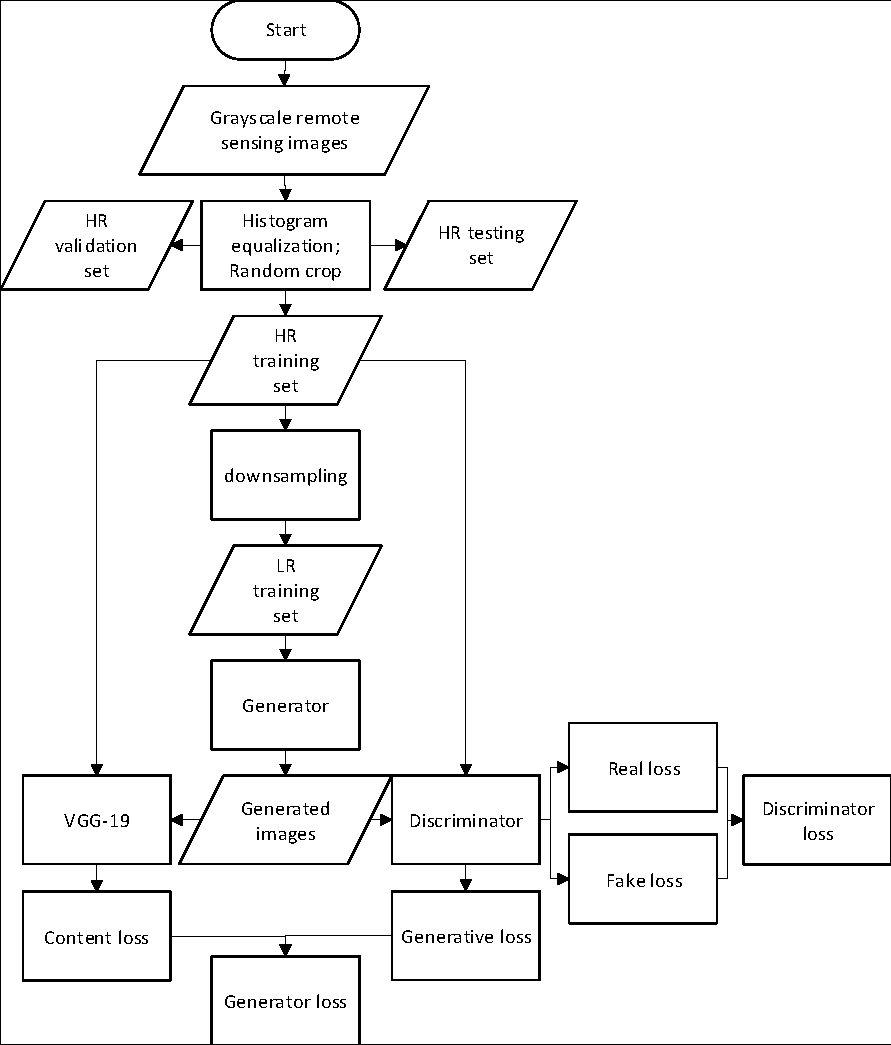
\includegraphics[width=0.8\textwidth]{fig1}
\end{center}
   \caption{Training flow chart of pbiSRGAN.}
\label{fig1}
\end{figure*}

 \begin{figure*}
\begin{center}
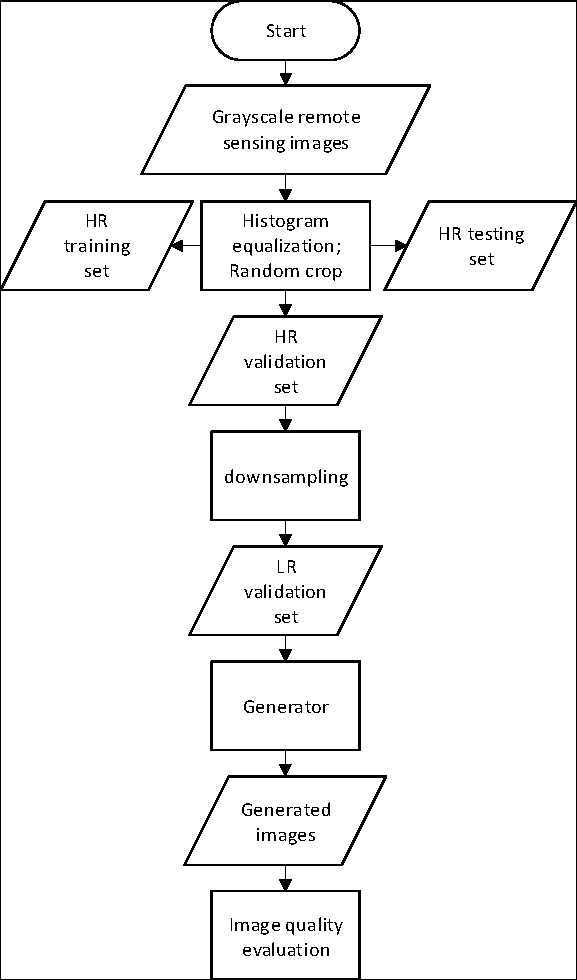
\includegraphics[width=0.5\textwidth]{fig2}
\end{center}
   \caption{Reconstructing flow chart of pbiSRGAN.}
\label{fig2}
\end{figure*}



{\small
\bibliographystyle{ieee_fullname}
\bibliography{egbib}
}

\end{document}
